\documentclass{sig-alternate}
\usepackage[latin1]{inputenc}
\usepackage{graphicx}        % standard LaTeX graphics tool
\usepackage{url} 
\usepackage{listings}
\usepackage{color}
% Style definition file generated by highlight 2.9, http://www.andre-simon.de/ 

% Highlighting theme definition: 

\newcommand{\hlstd}[1]{\textcolor[rgb]{0,0,0}{#1}}
\newcommand{\hlnum}[1]{\textcolor[rgb]{0.5,0,0.5}{\bf{#1}}}
\newcommand{\hlesc}[1]{\textcolor[rgb]{1,0,1}{\bf{#1}}}
\newcommand{\hlstr}[1]{\textcolor[rgb]{0.65,0.52,0}{#1}}
\newcommand{\hlpps}[1]{\textcolor[rgb]{0,0,1}{#1}}
\newcommand{\hlslc}[1]{\textcolor[rgb]{0.95,0.47,0}{#1}}
\newcommand{\hlcom}[1]{\textcolor[rgb]{1,0.5,0}{#1}}
\newcommand{\hlppc}[1]{\textcolor[rgb]{0,0.5,0.75}{\bf{#1}}}
\newcommand{\hlopt}[1]{\textcolor[rgb]{1,0,0.5}{\bf{#1}}}
\newcommand{\hlipl}[1]{\textcolor[rgb]{0.62,0.36,1}{#1}}
\newcommand{\hllin}[1]{\textcolor[rgb]{0.19,0.19,0.19}{#1}}
\newcommand{\hlkwa}[1]{\textcolor[rgb]{0.73,0.47,0.47}{\bf{#1}}}
\newcommand{\hlkwb}[1]{\textcolor[rgb]{0.5,0.5,0.75}{\bf{#1}}}
\newcommand{\hlkwc}[1]{\textcolor[rgb]{0,0.5,0.75}{#1}}
\newcommand{\hlkwd}[1]{\textcolor[rgb]{0,0.27,0.4}{#1}}
\definecolor{bgcolor}{rgb}{0.93,0.93,0.93}


\lstset{
basicstyle=\ttfamily \scriptsize,
language=java,
frame=single,
stringstyle=\ttfamily,
showstringspaces=false
}


\providecommand{\e}[1]{\ensuremath{\times 10^{#1}}}
\begin{document}
%
% --- Author Metadata here ---
\conferenceinfo{GECCO'13,} {July 6-10, 2013, Amsterdam, The Netherlands.}
    \CopyrightYear{2013}
    \crdata{TBA}
    \clubpenalty=10000
    \widowpenalty = 10000

\title{Developing services in a service oriented architecture for evolutionary algorithms}

%\subtitle{[Extended Abstract]
%\titlenote{A full version of this paper is available as
%\textit{Author's Guide to Preparing ACM SIG Proceedings Using
%\LaTeX$2_\epsilon$\ and BibTeX} at
%\texttt{www.acm.org/eaddress.htm}}}
%
% You need the command \numberofauthors to handle the 'placement
% and alignment' of the authors beneath the title.
%
% For aesthetic reasons, we recommend 'three authors at a time'
% i.e. three 'name/affiliation blocks' be placed beneath the title.
%
% NOTE: You are NOT restricted in how many 'rows' of
% "name/affiliations" may appear. We just ask that you restrict
% the number of 'columns' to three.
%
% Because of the available 'opening page real-estate'
% we ask you to refrain from putting more than six authors
% (two rows with three columns) beneath the article title.
% More than six makes the first-page appear very cluttered indeed.
%
% Use the \alignauthor commands to handle the names
% and affiliations for an 'aesthetic maximum' of six authors.
% Add names, affiliations, addresses for
% the seventh etc. author(s) as the argument for the
% \additionalauthors command.
% These 'additional authors' will be output/set for you
% without further effort on your part as the last section in
% the body of your article BEFORE References or any Appendices.


\numberofauthors{2}
 \author{
 \alignauthor
 Anonymous\\
        \affaddr{Lost island}\\
        \affaddr{Unknown}\\
        \affaddr{Pacific Ocean}\\
        \email{jack,sawyer,hurley@lost.com}
 \alignauthor
 Anonymous\\
 \affaddr{Lost island}\\
 \affaddr{Unknown}\\
 \affaddr{Pacific Ocean}\\
 \email{lock@lost.com}
 }

%\numberofauthors{2}
% \author{
% \alignauthor
% J.J. Merelo, A.M. Mora, C. M. Fernandes\\
%        \affaddr{University of Granada}\\
%        \affaddr{Department of Computer Architecture and Technology, ETSIIT}\\
%        \affaddr{18071 - Granada}\\
%        \email{jmerelo,amorag,cfernandes@geneura.ugr.es}
% \alignauthor
% Anna I. Esparcia-Alcázar\\
% \affaddr{S2 Grupo}\\
% \email{aesparcia@s2grupo.es}
% }


%\numberofauthors{4} %  in this sample file, there are a *total*
% of EIGHT authors. SIX appear on the 'first-page' (for formatting
% reasons) and the remaining two appear in the \additionalauthors section.
%

%\author{
% You can go ahead and credit any number of authors here,
% e.g. one 'row of three' or two rows (consisting of one row of three
% and a second row of one, two or three).
%
% The command \alignauthor (no curly braces needed) should
% precede each author name, affiliation/snail-mail address and
% e-mail address. Additionally, tag each line of
% affiliation/address with \affaddr, and tag the
% e-mail address with \email.
%
% 1st. author
%\alignauthor
%Jack\\
%       \affaddr{Lost island}\\
%       \affaddr{unknow}\\
%       \affaddr{Pacific Ocean}\\
%       \email{jack_the_doctor@lost.com}
% 2nd. author
%\alignauthor
%Sawyer\\
%       \affaddr{Lost island}\\
%       \affaddr{unknow}\\
%       \affaddr{Pacific Ocean}\\
%       \email{sawyer_tom@lost.com}
% 3rd. author
%\alignauthor 
%Lock\\
%       \affaddr{Lost island}\\
%       \affaddr{unknow}\\
%       \affaddr{Pacific Ocean}\\
%       \email{lock@lost.com}
% 4rd. author
%\alignauthor 
%Hurley\\
%       \affaddr{Lost island}\\
%       \affaddr{unknow}\\
%       \affaddr{Pacific Ocean}\\
%       \email{hugo@lost.com}
%}

%\and  % use '\and' if you need 'another row' of author names
% 4th. author
%\alignauthor Lawrence P. Leipuner\\
%       \affaddr{Brookhaven Laboratories}\\
%       \affaddr{Brookhaven National Lab}\\
%       \affaddr{P.O. Box 5000}\\
%       \email{lleipuner@researchlabs.org}
% 5th. author
%\alignauthor Sean Fogarty\\
%       \affaddr{NASA Ames Research Center}\\
%       \affaddr{Moffett Field}\\
%       \affaddr{California 94035}\\
%       \email{fogartys@amesres.org}
% 6th. author
%\alignauthor Charles Palmer\\
%       \affaddr{Palmer Research Laboratories}\\
%       \affaddr{8600 Datapoint Drive}\\
%       \affaddr{San Antonio, Texas 78229}\\
%       \email{cpalmer@prl.com}
%}
% There's nothing stopping you putting the seventh, eighth, etc.
% author on the opening page (as the 'third row') but we ask,
% for aesthetic reasons that you place these 'additional authors'
% in the \additional authors block, viz.
%\additionalauthors{Additional authors: John Smith (The Th{\o}rv{\"a}ld Group,
%email: {\texttt{jsmith@affiliation.org}}) and Julius P.~Kumquat
%(The Kumquat Consortium, email: {\texttt{jpkumquat@consortium.net}}).}
%\date{30 July 1999}
% Just remember to make sure that the TOTAL number of authors
% is the number that will appear on the first page PLUS the
% number that will appear in the \additionalauthors section.

\maketitle

\begin{abstract}
This paper shows a 
\end{abstract}

% A category with the (minimum) three required fields
\category{H.4}{Information Systems Applications}{Miscellaneous}
%A category including the fourth, optional field follows...
\category{G.1.6}{Mathematics of Computing}{NUMERICAL ANALYSIS}[Optimization]


%sures, performance measures
\terms{Algorithms}


\keywords{service oriented architecture, distributed algorithms, osgi}


%
%%%%%%%%%%%%%%%%%%%%%%%%%%%%%%%   INTRODUCTION   %%%%%%%%%%%%%%%%%%%%%%%%%%%%%%%
%
\section{Introduction}
\label{sec:intro}
%

%%CAMBIAR ESTO
When building quality software systems it is necessary to design them
with a high level of modularity. Besides the benefits that classic
modularization paradigms can offer (like object-oriented modelling)
and the improvements in test, reusability, availability and
maintainability, it is necessary to explore another modelling techniques, like the
plug-in based development \cite{PLUGINS}. This kind of development
simplifies aspects such as the complexity, personalization, configuration,
development and cost of the software systems. In the optimization
heuristics software area, the benefits the usage of this kind of
development can offer are carried out in the development of algorithms,
experimental evaluation, and combination of different optimization
paradigms \cite{PLUGINS}.  

On the other hand, other patterns for integration, like SOA, have emerged. SOA (Service Oriented Architecture) \cite{PAPAZOGLOU} is a paradigm for
organizing and utilizing distributed capabilities, called {\em services}. A service is an interaction depicted in Figure \ref{SOADIAGRAM}.

In our previous work \cite{OSGILIATH} we presente an abstract Service Oriented Architecture for Evolutionary Algorithms (SOA-EA), with guidelines and steps to migrate from traditional development to SOA. It also presents an specific implementation, called OSGiLiath: an environment for the development of distributed algorithms extensible via plug-ins architecture and based in a wide-accepted software specification (OSGi: Open Services Gateway Initiative \cite{OSGI}).

%\begin{figure}[ht] 
%\begin{center} 
%  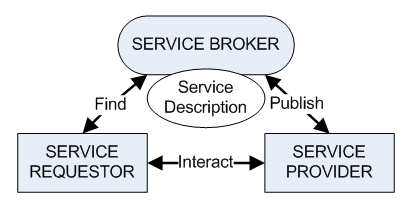
\epsfig{file=soaDiagram.eps,width=7.5cm} 
%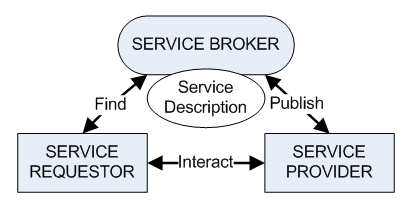
\includegraphics[scale=1]{soaDiagram.eps}
%\end{center} 
%\caption{Service interaction schema. The service provider publish a service description that is used by the requester to find and use services.} 
%\label{SOADIAGRAM} 
%\end{figure} 

The service provider publishes service descriptions (or interfaces) in the service registry, so the service requesters can discover services and bind to the service providers.



Distributed computing offers the possibility of taking advantage of parallel processing
 in order to obtain a higher 
computing power than other multiprocessor architectures. Two clear examples are the
research lines centred in clusters \cite{Buyya} and GRID \cite{GRID_ALGORITHMS}
for parallel processing. SOA it is also used in this area, using platforms based on Web Services \cite{PAPAZOGLOU}, and new standards for this paradigm have emerged, like OSGi.



Therefore, the objective of the proposed environment in this paper is to facilitate the
development of distributed computing applications by using the OSGi standard,
taking advantage
of the plug-in software development and SOA that can compete with existing
distributed applications in easy of use, compatibility and development.
The rest of the work is structured as follows: after the state of
the art, we present the developed algorithms and experimental setting. 
Then, the results of the experiments are shown (Section \ref{sec:results}), followed by conclusions and suggestions for future work.


%%%%%%%%%%%%%%%%%%%%%%%%%%%%%%  SOA  %%%%%%%%%%%%%%%%%%%%%%%%%%%%%%
%
\section{State of the art}
\label{sec:soa}
%
Even as SOA is used extensively in software development, it is not widely accepted in the main EA software. 

Nowadays there are many works about heuristic
frameworks. Most of them have the lack of low generality, because they
are focused in an specific field, like EasyLocal++ \cite{EASYLOCAL} (focused in Local Search) or
SIGMA \cite{SIGMA} (in the field of optimization-based decision support systems). Another common issue is that they are just libraries
 or Perl modules \cite{PERL}, they have no GUIs, or they are complicated to
install and require many programming skills. Another problem could be
the lack of comfort, for example, C++ has a more complicate sintaxis
than other languages. There also exist frameworks that use metaheuristics to apply in specific fields, like the KEEL framework \cite{KEEL}, that let the creation of heuristics to apply in data-mining problems.

Among this great number of frameworks we want to focus in the most widely accepted distributed algorithms frameworks. ECJ \cite{luke:ejb}, Evolutionary Computation in Java, is a set of Java classes that can be extended and includes several communication modules. MALLBA \cite{MALLBA} is based in software skelletons with a common and public interface. Every skeleton implements a resolution technique for optimization in the fields of exact, heuristic or hybrid optimization. It provides LAN and WAN capacity distribution with MPI . However, this both frameworks are not based in the plug-in development, so they can not take advantage of features like the life-cycle management, versioning, or dynamic service binding, as OSGi proposes.




Another important platform is DREAM \cite{LNCSDREAM}, which is an open source framework for Evolutionary Algorithms based on Java that
defines an island model and uses the Gossip protocol and TCP/IP sockets for
communication. It can be deployed in P2P platforms and it is divided
in five modules. Every module provides an user interface and different
interaction and abstraction level, but adding new functionalities is not so easy, due to the the fact that system must be stopped before adding new modules and the implementation of interfaces must be defined in the source code, so a new compilation is needed. OSGi lets the addition of new functionalities only compiling the new features, not the existing ones. 

Moreover, MALLBA and DREAM could be considered abandoned frameworks, due to no new publications or versions have been released. The MALLBA authors are now working in the jMetal Framework \cite{JMETAL}, that is a newer Java-based framework, but it has not yet distributed capabilities and it is focused in multi-objective optimization.

ParadiseEO \cite{PARADISE} allows the design of Evolutionary Algorithms and Local Search with hybridization, providing a variety of operators and evaluation functions. It also implement the most common parallel and distributed models, and it is based in standard libraries like MPI, PVM and Pthreads. However, it has the same problems that the previous frameworks, not lifecycle management or service oriented programming. GAlib \cite{GALIB} is very similar and share the same characteristics and problems.

In the field of the plug-in based frameworks, HeuristicLab \cite{HEURISTICLAB} is the most outstanding example. It also allows the distributed programming using Web Services and a centralized database, instead using their own plug-in design for this distributed communication. 

HeuristicLab \cite{HEURISTICLAB} is one of the few plug-in and service oriented frameworks. It uses web services for communication, but just to distribute the load, after consulting a central database of available jobs.

Finally, METCO framework \cite{METCO} also have the same problems, it does not use a standard plug-in system or SOA, but let the implementation of existing interfaces, and lets the user configure its existing functionalities.



Finally, the only service oriented optimization framework is GridUFO \cite{GRIDUFO}, but it only allows the modification of the objective function and the addition of whole algorithms, without combining existing services. 

\section{Service Oriented Architecture in Evolutionary Algorithms}
Previous sections have demonstrated that it is possible to create a service oriented architecture for EAs using a specific SOA technology. This architecture uses the features that SOA offers. To do this:
In summary, the previous works present a number of shortcomings when designing and adding new features: they need to modify source code or be stopped in order to add new features and they are not based in a public plug-in specification. Also they have not an event administration mechanism and they are not service-oriented, so they not take advantage of this paradigm.
\begin{itemize}
\item In Sections \ref{sec:soa4eas} and \ref{sec:examples} loose coupling services for EAs have been designed (SOA-EA), and they have been implemented in Section \ref{sec:osgiliath}.
\item These services can be combined in several ways to obtain different algorithms (from a canonical GA, a NSGA-II has been created just adding new services). These services are dynamically bound to cha\-nge the needed EA aspects. The source code of  the basic EA services have not been re-written or re-compiled to achieve this task.
\item New services can be added in execution time using our implementation.
\item No specific source code for a basic distribution have been added, neither the existing source code has been modified.
\item Several techniques have been presented to combine existing services in a flexible way.
\end{itemize}


However, after the explanation of the most important issues of EAs in SOA (Algorithm representation, dynamism, load distribution and self-adapting), we want to share  the benefits of SOA with the rest of EA researchers:

% estás repitiendo lo mismo que dijiste antes, sin una prueba ni
% comparación! - JJ
% FERGU: hombre, la prueba es el código fuente que está en el SVN.

\begin{itemize}
\item Firstly, SOA fits with the genericity advantages in the development of software for EAs \cite{GENERICITY05} and adds new features, like language independence and  distribution mechanisms.
\item SOA allows the addition and removal of services in execution time without altering the general execution of the algorithm (that is, it is not mandatory to stop it or to add extra code to support new operators).
\item It also increases the interoperability between different software elements (for example, it is possible to add communication libraries without modifying existing code).
\item Related to the previous point, the existing EA frameworks could be re-used thanks to SOA, because it provides language independence.
\item Easiness for code distribution: SOA does not require the use of a concrete implementation or library.
\item Access to already created and operative services.% (as previously stated STATService for non-parametric tests).
\item Collaboration among geografically distributed work teams.
\end{itemize}

\section{Implementation technology}
This section dives into some technical features of the OSGi platform, to guide the reader to understand the OSGiLiatH framework in a deeper way, and to evaluate the advantages of using this features in the development of distributed algorithms.

OSGi (Open Service Gateway Initiative) \cite{OSGI} was proposed by a consortium of more than
eighty companies in order to develop an infrastructure for the
deployment of service in heterogeneous network of devices, mainly
oriented to domotics \cite{OSGIOVERVIEW}. Nowadays it defines a
specification for a Service Oriented Architecture for virtual
machines (VMs). It provides very desiderable features, like
packet abstraction, life-cycle management, packaging or versioning,
allowing significant reduction of the building, support and deployment
complexity of the applications. 

OSGi technology allows dynamic discovery of new components, to increase the collaboration and to minimize and manage the coupling
among modules. Moreover, the
OSGi Alliance has developed several standard component interfaces for
common usage patterns, like HTTP servers, configuration, logs, security,
management or XML management among others, whose implementations can
be obtained by third-parties. Nowadays there are some challenges 
in the OSGi development \cite{OSGICHALLENGES}, but they only affect the creation of very complex applications.

This advantages are not so
                               costly, as can be thought: the OSGi
                                framework can be implemented in a
                                {\em jar} file\footnote{A jar file is
                                a file that groups the compiled Java
                                files.} of 300KB. Also, and different
                                of the normal usage of Java, each
                                class pre-charges only the other
                                classes to use, not all. Also is
                                non-intrusive: the code to be
                                executed in OSGi can be executed
                                without it. Finally, from its
                                specification in 1998 has been widely
                                used as base in big projects: the
                                Eclipse IDE (Integrated Development
                                Environment) is built over OSGi, and
                                also big application servers
                               (Glassfish or IBM Websphere) or
                               residential gateways
                               \cite{OSGIGATEWAY}, among other
                               examples. 

\subsection{OSGi Architecture}
To understand how OSGi \cite{OSGI} works and which capabilities could offer to the OSGiLiath users it is necessary to understand how OSGi is built. OSGi has a layered model that is depicted in Figure \ref{fig:osgi-original}. The terms present in this Figure are:

\begin{itemize}
\item Bundles: Bundles are the OSGi components made by developers (explained in previous sections).
\item Services: This layer connects bundles in a dynamic way by offering a publish-find-bind model.
\item Life-Cycle: The API to install, start, stop, update, and uninstall bundles.
\item Modules: This layer defines how a bundle can import and export code (using the MANIFEST.MF file).
\item Security: Security aspects are handled in this layer.
\item Execution Environment: Defines what methods and classes are available in a specific platform. For example, mobile devices have less Java classes due to performance constraints.
\end{itemize}


\begin{figure}[t] 
\begin{center} 
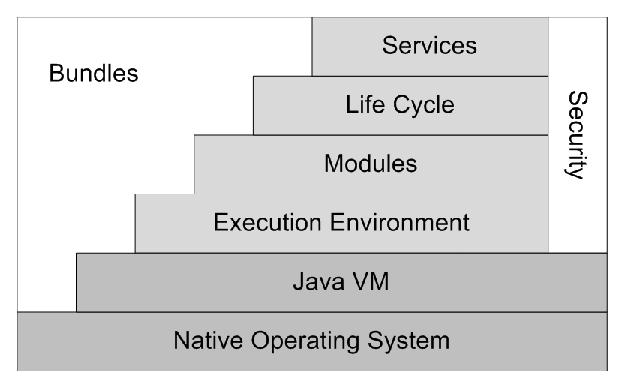
\includegraphics[scale=0.8]{images/osgi-oficial.eps} 
\end{center} 
\caption{OSGi layered architecture. Every layer is built from the one just below.} 
\label{fig:osgi-original} 
\end{figure}


\subsection{OSGi configuration files}
Regarding to explained OSGi layers how to use all OSGi capabilities is shown next. Java programmers are familiar with the {\em jar} concept. The first difference among a {\em bundle} and a {\em jar} is that the second has a MANIFEST.MF file adapted to be used in OSGi. This file indicates which clasess imports or exports the {\em bundle}. An example can be seen in Figure \ref{fig:manifest}. This file shows the name of the bundle and its version (this is useful to select specific services), and the execution environment (that is, the Java Virtual Machine required). Also, this file specifies the XML files of the declarative services (in section ({\em Service-Component}).

\begin{figure}[t]
\noindent
\ttfamily
\hlstd{}{\bf Manifest-Version:} 1.0\\
\hlstd{}{\bf Bundle-ManifestVersion:} 2\\
\hlstd{}{\bf Bundle-Name:} GeneticAlgorithm Plug-in\\
\hlstd{}{\bf Bundle-SymbolicName:} geneticalgorithm\\
\hlstd{}{\bf Bundle-Version:} 1.0.0\\
\hlstd{}{\bf Bundle-RequiredExecutionEnvironment:} J2SE-1.5\\
\hlstd{}{\bf Import-Package:} ch.ethz.iks.r-osgi,\\
 \hlstd{}es.ugr.osgiliath.algorithms,\\
 \hlstd{}es.ugr.osgiliath.algorithms.types,\\
 \hlstd{}es.ugr.osgiliath.network,\\
 \hlstd{}es.ugr.osgiliath.problem,\\
 \hlstd{}es.ugr.osgiliath.utils,\\
  \hlstd{}org.osgi.framework\\
\hlstd{}{\bf Export-Package:} es.ugr.osgiliath.geneticalgorithm,\\
 \hlstd{}es.ugr.osgiliath.geneticalgorithm.distributed\\
  \hlstd{}es.ugr.osgiliath.geneticalgorithm.individual\\
   \hlstd{}es.ugr.osgiliath.geneticalgorithm.operators\\
\hlstd{}\hlkwa{Service-Component:} OSGI-INF/distributedGA.xml\\
\mbox{}
 
\normalfont
\label{fig:manifest}
\caption{Example of MANIFEST.MF. This example defines which packages are necessary to activate the bundle and which packages are exported.}
\end {figure}

As can be seen in previous sections, it is in the second and third level of the development in OSGiLiatH where the declarative services specification is used to automatically obtain the implementation of the interfaces. In normal environments, to create an specific implementation of an interface (i.e. {\em ObjectiveFunction}) is as follows:

\begin{lstlisting}
class GeneticAlgorithm implements Algorithm{
 ObjectiveFunction obj;
 //A new instance is bind to a reference
 ObjectiveFunction f = new ExampleFunction();
}
\end{lstlisting}
 
With Declarative Services, the {\em new Implementation()} part is not necessary. For example, Figure \ref{fig:ds} shows a service component file, which stablish in execution time which implementation is bound to the interfaces. This example indicates that the implementation of service {\em Algorithm} is {\em GeneticAlgorithm}, but this service is not activated until all their references (other services, like {\em ObjectiveFunction} or {\em Crossover}) are also activated. The tag {\em cardinality} means that at least one service of that kind must exist (the first {\em 1} represents optionality) and  the second part (the other {\em 1} indicates the number of different implementations that can be managed: one ({\em 1}) or many ({\em *}). The file where these capabilities are defined is declared in section {\em Service-Component} of MANIFEST.MF file, as can be seen in Figure \ref{fig:manifest}.
\begin{figure}[t]
\noindent
\ttfamily

\hlstd{}\hlkwa{$<$?xml\ }\hlstd{}\hlkwb{version}\hlstd{=}\hlstr{"1.0"}\hlstd{}\hlkwa{?$>$}\hspace*{\fill}\\
\hlstd{}\hlkwa{$<$component\ }\hlstd{}\hlkwb{name}\hlstd{=}\hlstr{"geneticalgorithm"}\hlstd{}\hlkwa{$>$}\hspace*{\fill}\\
\hlstd{\ }\hlkwa{$<$implementation}\hspace*{\fill}\\
\hlstd{}\hlstd{\ \ }\hlstd{}\hlkwb{class}\hlstd{=}\hlstr{"es.ugr.osgiliath.geneticalgorithm.GeneticAlgorithm"}\hlstd{}\hlkwa{/$>$}\hspace*{\fill}\\
\hlstd{\ }\hlkwa{$<$service$>$}\hspace*{\fill}\\
\hlstd{}\hlstd{\ \ }\hlstd{}\hlkwa{$<$provide}\hspace*{\fill}\\
\hlstd{}\hlstd{\ \ \ }\hlstd{}\hlkwb{interface}\hlstd{=}\hlstr{"es.ugr.osgiliath.algorithms.Algorithm"}\hlstd{}\hlkwa{/$>$}\hspace*{\fill}\\
\hlstd{\ }\hlkwa{$<$/service$>$}\hspace*{\fill}\\
\hlstd{\ }\hlkwa{$<$reference\ }\hlstd{}\hlkwb{name}\hlstd{=}\hlstr{"OBJECTIVEFUNCTION"}\hlstd{\hspace*{\fill}\\
}\hlstd{\ \ }\hlstd{}\hlkwb{interface}\hlstd{=}\hlstr{"es.ugr.osgiliath.geneticalgorithm.ObjectiveFunction"}\hlstd{\hspace*{\fill}\\
}\hlstd{\ \ }\hlstd{}\hlkwb{bind}\hlstd{=}\hlstr{"setObjectiveFunction"}\hlstd{\hspace*{\fill}\\
}\hlstd{\ \ }\hlstd{}\hlkwb{unbind}\hlstd{=}\hlstr{"unsetObjectiveFunction"}\hlstd{\hspace*{\fill}\\
}\hlstd{\ \ }\hlstd{}\hlkwb{cardinality}\hlstd{=}\hlstr{"1..1"}\hlstd{}\hlkwa{/$>$}\hspace*{\fill}\\
\hlstd{\ }\hlkwa{$<$reference\ }\hlstd{}\hlkwb{name}\hlstd{=}\hlstr{"PARAMETERS"}\hlstd{\hspace*{\fill}\\
}\hlstd{\ \ %}\hlstd{}\hlkwb{interface}\hlstd{=}\hlstr{"es.ugr.osgiliath.algorithms.Parameters"}\hlstd{\hspace*{\fill}%\\
}\hlstd{\ \ }\hlstd{}\hlkwb{bind}\hlstd{=}\hlstr{"setParameters"}\hlstd{\hspace*{\fill}\\
}\hlstd{\ \ }\hlstd{}\hlkwb{unbind}\hlstd{=}\hlstr{"unsetParameters"}\hlstd{\hspace*{\fill}\\
}\hlstd{\ \ }\hlstd{}\hlkwb{cardinality}\hlstd{=}\hlstr{"1..1"}\hlstd{}\hlkwa{/$>$}\hspace*{\fill}\\
\hlstd{\ }\hlkwa{$<$reference\ }\hlstd{}\hlkwb{name}\hlstd{=}\hlstr{"CROSSOVER"}\hlstd{\hspace*{\fill}\\
}\hlstd{\ \ }\hlstd{}\hlkwb{interface}\hlstd{=}\hlstr{"es.ugr.osgiliath.geneticalgorithm.operators.Crossover"}\hlstd{\hspace*{\fill}\\
}\hlstd{\ \ }\hlstd{}\hlkwb{bind}\hlstd{=}\hlstr{"setCrossover"}\hlstd{\hspace*{\fill}\\
}\hlstd{\ \ }\hlstd{}\hlkwb{unbind}\hlstd{=}\hlstr{"unsetCrossover"}\hlstd{\hspace*{\fill}\\
}\hlstd{\ \ }\hlstd{}\hlkwb{cardinality}\hlstd{=}\hlstr{"1..1"}\hlstd{}\hlkwa{/$>$}\hspace*{\fill}\\
\hlstd{\ }\hlcom{$<$!{-}{-}\ Rest\ of\ references\ ...{-}{-}$>$}\hlstd{}\hspace*{\fill}\\
\hlkwa{$<$/component$>$}\hlstd{}\hspace*{\fill}\\
\mbox{}

\normalfont
\label{fig:ds}
\caption{Service Description. This documents indicates that the implementation of the service {\em Algorithm} is {\em GeneticAlgorithm}, but it can not activate until their references (other services) are activated.}
\end {figure}

This document indicates that the implementation of the service {\em Algorithm} is the class {\em GeneticAlgorithm}, but it can not be activated until the rest of the references (another services, like {\em Crossover}) are activated first. We need to create XML files for the rest of services to use (i.e. ObjectiveFunction)

\begin{lstlisting}
class GeneticAlgorithm implements Algorithm{
 //Other service references, like Crossover, Parameters...
 ObjectiveFunction obj;
 
 //Methods to bind/unbind each reference
 public ObjectiveFunction setObjectiveFunction(ObjectiveFunction obj){
  this.obj = obj;
 }
	
 public void unsetObjectiveFunction(ObjectiveFunction obj){
  this.obj = null;
 }
}
\end{lstlisting}

We have to say that in future work these kind of files will be automatically created, being this task transparent to future users of the OSGiLiatH framework.

\subsection{Event Administration}
The Event Administration in OSGi lets the usage of a blackboard communitacion architecture where bundles can broadcast or receive events without notice which bundles are sending or receiving these events.

%Acquire a reference to the EventAdmin OSGi service, it implements the org.osgi.service.event.EventAdmin.
%Pick a topic name for the event and make sure that it follows Topic Naming Conventions mentioned above.
%Fill Event Properties in a dictionary that will be passed as a parameter to the publish method.
%Having the Topic Name and Properties, ready invoke one of the following methods of the Event Admin service: postEvent or sendEvent - while postEvent initiates synchronous delivery of the event, sendEvent initiates asynchronous delivery of the event. So by default, your option should be postEvent method unless you have strict requirements to not continue execution until all handlers of the event handle it.

To send events to other bundles:
\begin{itemize}
\item Acquire a reference to the EventAdmin OSGi service (via Declarative Services, for example).
\item Pick a topic name for the event (for example {\em ``es/ugr/osgiliath/algorithms/geneticalgorithm/endgeneration''})
\item Send the event using the {\em postEvent} method of EventAdmin, with the topic plus other desired properties %(poner lo de sincrono/asincrono?)
\end{itemize}

Code to send an event to other bundles is shown below. The programmer specifies the topic String and optional properties to send to other bundles that are listening. The {\em eventAdmin} variable is a reference to {\em ``org.osgi.service.event. EventAdmin''} service, obtained via Declarative Services or by hand (not showed).

\begin{lstlisting}
Properties props = new Properties(); //Optional
String topic = "es/ugr/osgiliath/algorithms/geneticalgorithm/endgeneration";
Event evt = new Event(topic,props);
eventAdmin.postEvent(evt);
\end{lstlisting}
		
For the other hand, the steps to handle events are:
\begin{itemize}
\item Register a service that implements the OSGi EventHandler interface (via Declarative Services or manually).
\item Specify in this service the topics to subscribe to. For example, the String {\em ``es/ugr/osgiliath/algorithms/geneticalgorithm/*''} (the * is a wildcard) inside the $<$property$>$ tag in the Service Component.
\item Overwrite the handleEvent method of this interface with the desired code.
\end{itemize}

This code shows how to handle events. In this case we have published the {\em ExampleService} with the implementation {\em ExampleImpl}, that is listening under the topic {\em ``es/ugr/osgiliath/algorithms/geneticalgorithm/*''}.

\begin{lstlisting}
class ExampleImpl implements ExampleService,EventHandler{

 public void handleEvent(Event ev){
  if(evt.getTopic().endsWith("endgeneration")){
   // An event with topic 
   // "es/ugr/osgiliath/algorithms/geneticalgorithm/endgeneration"
   System.out.println("Generation over");
  else{
   // Other event with topic starts with
   // "es/ugr/osgiliath/algorithms/geneticalgorithm/"
   System.out.println("Other event received");
  }
 }
}
\end{lstlisting}

%%%%%%%%%%%%%%%%%%  DEVELOPMENT  %%%%%%%%%%%%%%%%%%%

\subsection{Distribution}
In OSGiLiath all services can be distributed using the OSGi features. In this case, the distribution is performed using the service descriptor to set which service is distributable and which is the distribution technology that provides service discovering and data transmission.

OSGi allows several implementations for the service distribution. ECF\footnote{\url{http://www.eclipse.org/ecf/}} has been chosen because it is the most mature and accepted implementation \cite{petzold2011dynamic}, and it also supports the largest number of transmission protocols, including both synchronous and asynchronous communication. It provides a modular implementation of the OSGi 4.2 Remote Services standard \footnote{\url{http://www.osgi.org/Release4/Download}}. This specification uses the OSGi service registry to expose remote services.. ECF also separates the source code from the discovery and transmission mechanism, allowing users to apply the most adequate technology to their needs, and providing the integration with existing applications. % For example, the lines of Figure \ref{fig:remote} have been added to the service descriptor of {\em MOP2 Fitness Calculator} to distribute it in the local network.

ECF includes a number of protocols for service discovery and service providers:
\begin{itemize}
\item Service Discovery API: Includes protocols to announce and discover remote services: Zeroconf, SLP/RFC 2608, Zookeeper, file-based and others
\item Service Provider API: Includes protocols to establish the communication (data streams, formats and others): R-OSGi, ActiveMQ/JMS, REST, SOAP, XMPP, ECF Generic
\end{itemize}

\section{OSGiLiath}
This section explains the functionality and design of the proposed environment, called OSGiLiatH ({\em OSGi Laboratory for Implementation and Testing of Heuristics}). This environment is a  framework for the development of heuristic optimization applications, not centred on a concrete paradigm, and whose main objective is to promote the OSGi and SOA usage and offer to programmers the next features:

\begin{itemize}
\item Easy interfaces. After a study of the previous frameworks a complete interface hierachy has been developed.
\item Asynchronous data sending/receiving. Thanks to R-OSGi distributed capabilities, the framework has easy distribution of services, without implementing specific source functions, like MPI or other distribution frameworks. Programmers do not need to write communication code. 
\item Component Oriented Programming. The framework is plug-in oriented, so new improvements can be added in easy way without modification of existent modules. Adding o modifying implementations of services can be performed without re-compilation of the source code.
\item Client/Server or Distributed Model. All components of the framework can communicate in a bi-directional way, so a central broker is not necessary if it is not required.
\item Paradigm independent. The framework is not focused in a type of metaheuristic.
\item Declarative Services. Bind interfaces to specific implementations can be done without modifying existent source code. Programmers do not need to instantiate implementations of the services.
\item Remote event handling: Using the OSGi and R-OSGi advantages, users can use a powerful tool to synchronize or share data among services.
\end{itemize}

The source code is available at \url{http://atc.ugr.es/~pgarcia}, under a GPL license.

\subsection{OSGiLiath organization}
By now, OSGiLiath counts with the next bundles:

\begin{itemize}
\item osgiliath: This is the core bundle. It includes all the interfaces common to the algorithms such as...
\item Evolutionary Algorithm: Evolutionary Algorithm implementation and interfaces to create the rest of Recombinator and Crossover, Mutator and Mutation, TERMINA. It also provides interfaces for the creation of individuals: Individual, Fitness, Gene, Genome, 
\item Basic Evolutionary Components: Includes several implementations of the previous interfaces: 
\item Binary Problems: Includes implementation of well-known problems, such as OneMax and MMDP, with INDIVIDUALS tal...
\item Function Problems: 
\item NSGA2: 
\item OSGiLiART: Service implementation for the creation of Evolutionary Art.
\item NoOSGi: Because OSGi allows the separation of source code with the OSGi framework capabilities, this bundle includes Java code to integrate the services without any specific technology (just basic Object Oriented programming).
\item IntelligentManager: An example of how the services can be bound/unbound in real-time. By now, in each step the IntelligentRandomManager hace PATATIN Y PATATAN.
\end{itemize}

\section{Development of service}
\label{sec:development}
This section presents the steps to add services to the existent OSGiLiath core.

\subsection{Bundle creation}

\subsection{Implementing services}



\section{Conclusions}



%ACKNOWLEDGMENTS are optional
\section{Acknowledgments}
This work has been supported in part %by FPU research grant AP2009-2942 and projects AmIVital (CENIT2007-1010), EvOrq (P08-TIC-03903), UGR PR-PP2011-5 and TIN2011-28627-C04-02.

%
% The following two commands are all you need in the
% initial runs of your .tex file to
% produce the bibliography for the citations in your paper.


%\bibliographystyle{abbrv} CAMBIAR!!!!!!
\bibliographystyle{plain}
\bibliography{osgi-evosoft}  % sigproc.bib is the name of the Bibliography in this case


\end{document}
